\documentclass[a4paper,10pt]{article}
\usepackage[a4paper,left=15mm,right=15mm,top=20mm,bottom=20mm]{geometry}  % 設置頁面的環境, a4紙張大小,左右上邊距信息
\usepackage{indentfirst}  %用首行縮排要引入這個
\usepackage{physics}  %用 braket 用引入這個
%\usepackage{amsmath}  %用矩陣用引入這個
\usepackage{graphicx}  %插入圖片用這個
\usepackage{mathtools}
\usepackage{cancel}
\usepackage{bm}
\allowdisplaybreaks[4]
 \setlength{\parindent}{2em}

\title{Computational Astrophysic\\Homework 4}
\author{d07222009 Guan-Ming Su}
\date{\today}       %日期

\begin{document}

\maketitle

%标题开始
\section*{Theorem}
\begin{large}
In this problem, we conduct a convolution operation on the given input picture using a Gaussian filter of size $N\times N$  (same as the input picture size) to generate the output image:
\begin{align*}
O_{i,j}=\sum_k\sum_lI_{k,l}F_{[i-k],[j-l]},
\end{align*}
where $N=1024$, $O_{i,j}$ is the pixel of row i column j, $I_{kl}$ is the pixel of the input picture of row k column l, and $F_{[i-k],[j-l]}$ is the pixel of the Gaussian filter at row $(i-k)$ mod($N$) and column $(j-l)$ mod($N$). The component $F_{[i-k],[j-l]}$ is contructed according to:
\begin{align*}
F_{[i-k],[j-l]} = Ae^{-\frac{[i-k]^2}{2\sigma^2}}e^{-\frac{[j-l]^2}{2\sigma^2}}=\frac{e^{-\frac{[i-k]^2}{2\sigma^2}}e^{-\frac{[j-l]^2}{2\sigma^2}}}{\sum_{[i-k]}\sum_{[j-l]}e^{-\frac{[i-k]^2}{2\sigma^2}}e^{-\frac{[j-l]^2}{2\sigma^2}}},
\end{align*}
A is the normalization constant.


Instead of using direct integration, the matrix $O_{i,j}$ can be calcualted efficient by discret Fourier transform, as proven below:
\begin{align}\notag
O_{k_\alpha,k_\beta}&=\sum_{i}\sum_{j}O_{i,j}e^{ik_\alpha i}e^{ik_\beta j} = \sum_k\sum_lI_{k,l}e^{ik_\alpha k}e^{ik_\beta l}\sum_i\sum_jF_{[i-k],[j-l]}e^{ik_\alpha [i-k]}e^{ik_\beta [j-l]}=I_{k_\alpha,k_\beta}F_{k_\alpha,k_\beta}\\
&\Rightarrow O_{i,j}=\frac{1}{N^2}\sum_{k_\alpha}\sum_{k_\beta} I_{k_\alpha,k_\beta}F_{k_\alpha,k_\beta}e^{-ik_\alpha i}e^{-ik_\beta j}.
\end{align}
Thus, by calculating the 2D discret Fourier transform of both input picture as well as the Gaussian filter, the output image can be easily produced by conducting inverse Fourier transform on the multiply of them.
\end{large}
\section*{Output Images and Power Spectrums}
\begin{large}
The output images were generated following Eq. (1) using the FFT package of numpy;  the power spectrums are obtaine by taking the square of amplitude of the output image Fourier comonents, and plotted in log scale, i.e. $log(\left |O_{k_\alpha,k_\beta}\right |^2)=2log(\left |O_{k_\alpha,k_\beta}\right |)$.\\

Since the Gaussian filter is nothing but producing a image with pixel $O_{i,j}$ by averaging over the input picture (set $I_{i,j}$ as center) with a normal distribution weight function, so effect is quite similiar to averaging a region of size $(\sigma,\sigma)$ with unifrom distribuion, where $\sigma$ is the variance of the normal distribution, one expects that the output image should be delicate with more details preserved when $\sigma$ is small, while become more rough but the large scale trend will be extracted if $\sigma$ is large. Accordingly, when $\sigma$ is small, the power spectrum will contain stronger short wave length (high $k$) modes which is essential for constructing the local structures; for large $\sigma$, only the long wave length (low $k$) modes survive since all the detail structures have been smeared out.
\begin{figure}[htbp] %htbp 代表图片插入位置的设置
\centering %圖片置中
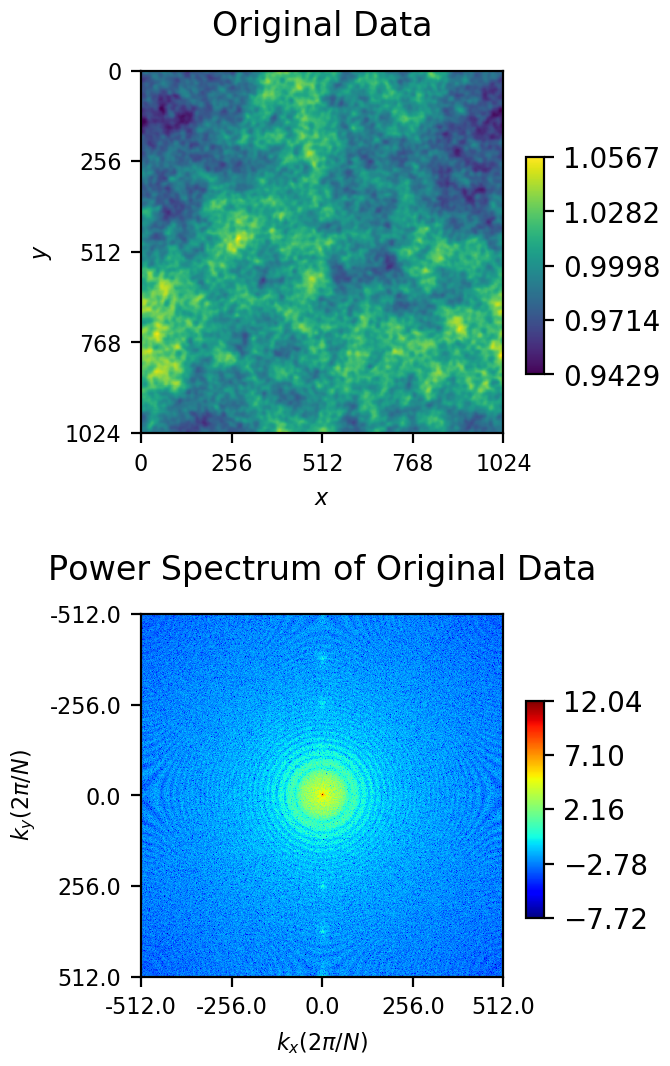
\includegraphics[width=13cm]{original.png} %[]可選參數,控制圖片大小
%圖片說明
\caption{Density Distribution and Power Spectrum for Original Data}
\end{figure}

\begin{figure}[htbp] %htbp 代表图片插入位置的设置
\centering %圖片置中
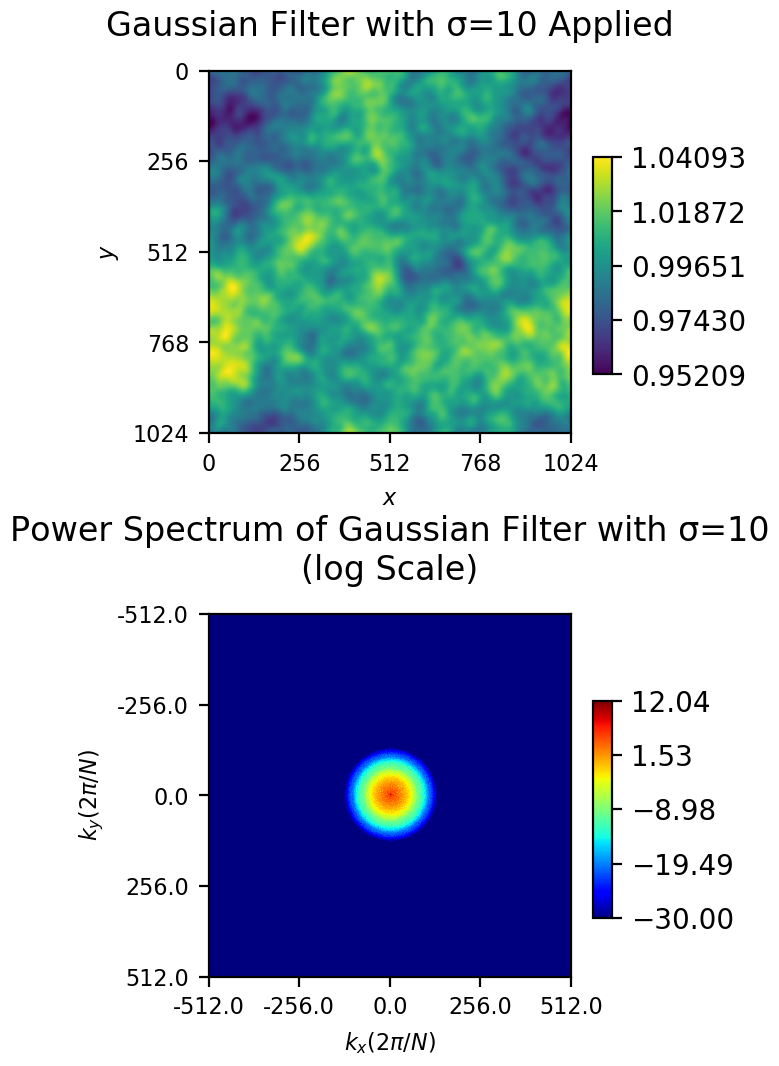
\includegraphics[width=14cm]{sigma=10.png} %[]可選參數,控制圖片大小
%圖片說明
\caption{Density Distribution and Spectrum Density for $\sigma=10$ Gaussian Filter}
\end{figure}

\begin{figure}[htbp] %htbp 代表图片插入位置的设置
\centering %圖片置中
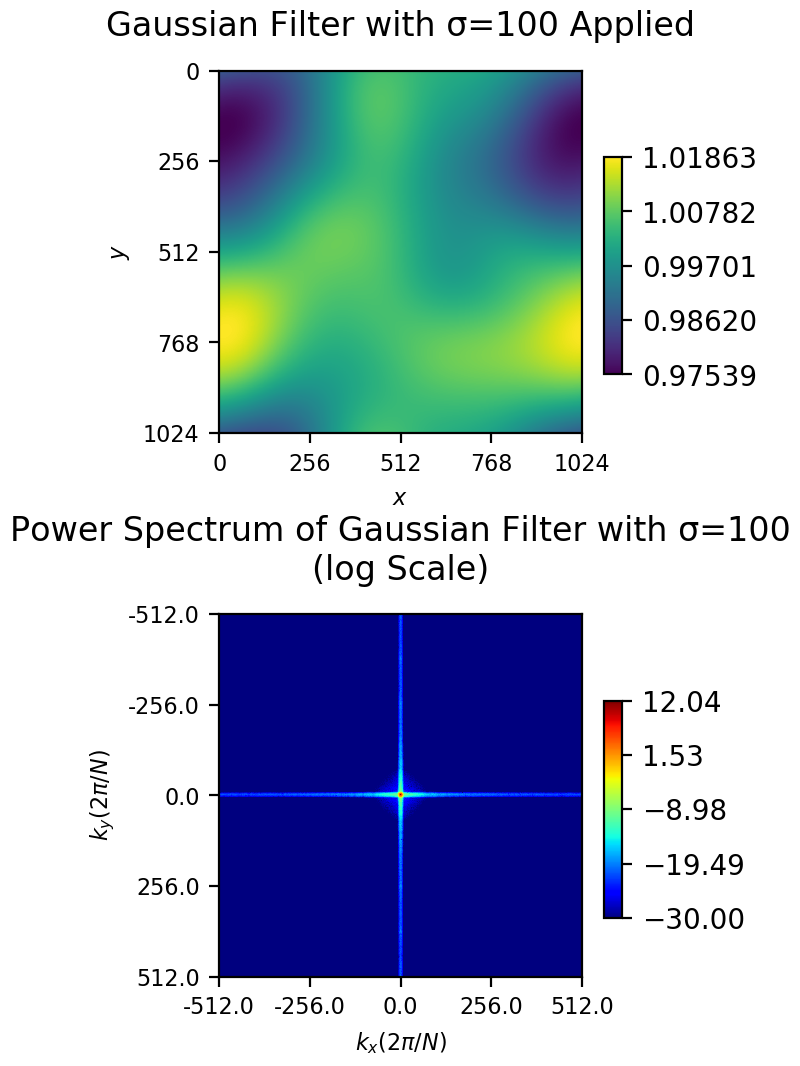
\includegraphics[width=14cm]{sigma=100.png} %[]可選參數,控制圖片大小
%圖片說明
\caption{Density Distribution and Spectrum Density for $\sigma=100$ Gaussian Filter}
\end{figure}

\end{large}

\newpage
\section*{Discussion}
\begin{large}
The result clearly shows that our expectation is correct: the output image becomes more and more blurring from original data to be filtered by $\sigma=10$  and then by $\sigma=100$. Since we average over a wider region when $\sigma$ is large, if a histogram of each pixel value is plotted, one should expect that bars of histogram become more centralized, due to lost of details and averging with lots of other pixels, which is confirmmed by in Fig. 4. \\
\begin{figure}[htbp] %htbp 代表图片插入位置的设置
\centering %圖片置中
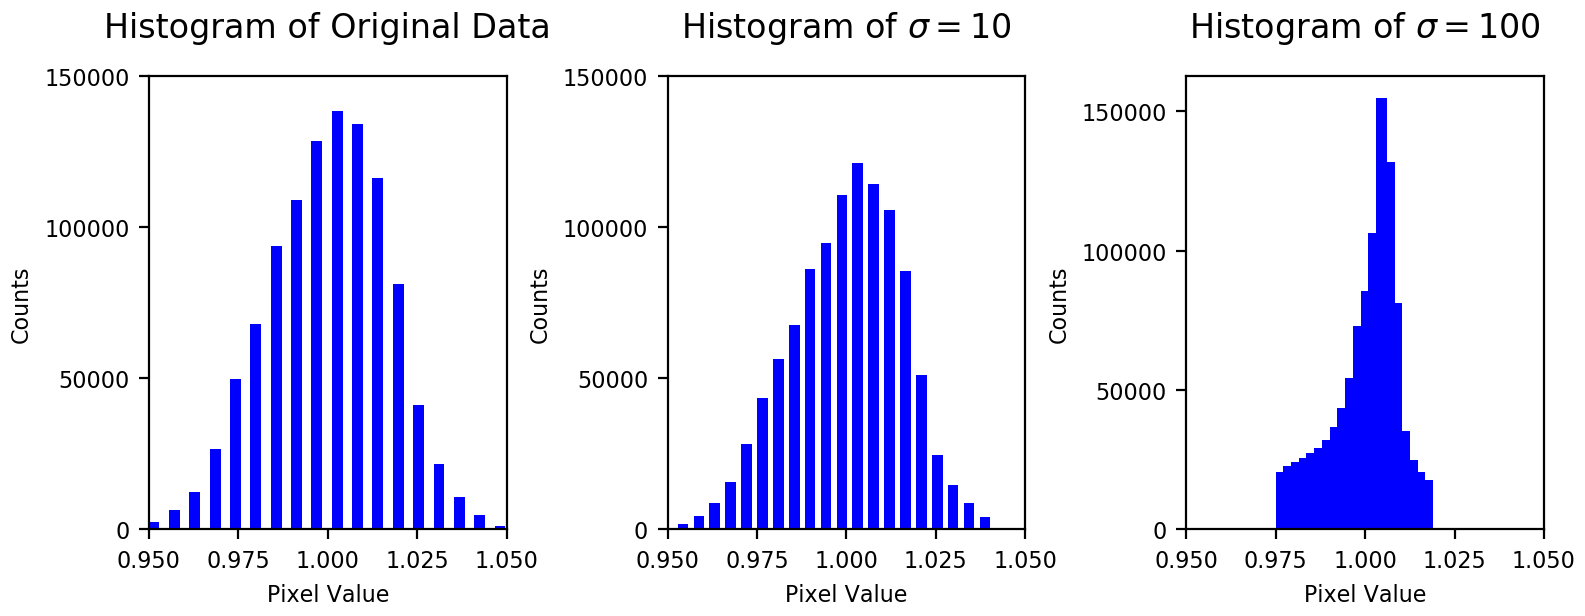
\includegraphics[width=13cm]{pixel_value_histogram.png} %[]可選參數,控制圖片大小
%圖片說明
\caption{Histogram of Pixel Value for Original Data and Filtered Output}
\end{figure}

As for the power spectrum, we truncated modes whose square of norm is below $10^{-30}$ and filled them with $10^{-30}$. It can observed that for the original data, though the dominant components are centered around  $(0,0)$ of $k_x-k_y$ plane, there are considerable modes extend to high $k$ region with certian patterns (nearly four-fold symmetry), and no mode is truncated, i.e., various of modes contribute to the input image. For $\sigma=10$ filter, we see most of the modes are truncated except a cricle around the origin with radius $\approx128\frac{2\pi}{N}$, suggesting only short k modes are preserved. For $\sigma=100$, the surviving modes are centered in a way narrow circle, and the original cylindrical in $\sigma=10$ case is broken into four-fold symmetry, with a cross situates at the center. I guess this cross comes from some $x$ symmetry and $y$ symmetry regions in the output image (shown in Fig. 5). To quantify how the surviving modes change with the $\sigma$, the variance of $k_x$ and $k_y$ is calcuated by:
\begin{align*}
\begin{cases}
&var(k_x)=\sqrt{A\sum_{k_\alpha}\sum_{k_\beta}O_{k_\alpha,k_\beta}k_\alpha^2-(A\sum_{k_\alpha}\sum_{k_\beta}O_{k_\alpha,k_\beta}k_\alpha)^2} \\
&var(k_x)=\sqrt{A\sum_{k_\alpha}\sum_{k_\beta}O_{k_\alpha,k_\beta}k_\beta^2-(A\sum_{k_\alpha}\sum_{k_\beta}O_{k_\alpha,k_\beta}k_\beta)^2}\\
\end{cases},
\end{align*}
where $A=\sum_{k_\alpha}\sum_{k_\beta}O_{k_\alpha,k_\beta}$. As shown in table 1 and Fig. 6, the variance does decrease with increasing $\sigma$.

\begin{table}[h]  %table 里面也可以嵌套tabular,只有tabular是不能加标题的
\centering  %表格居中
\begin{tabular}[t]{|c|c|c|c|}
\hline
$\sigma$ &$ var(k_x)$ & $var(k_y)$\\
\hline
Original&58.20387650&58.87456062\\
\hline
10&4.86205933&4.85042083\\
\hline
100&0.22526556&0.22104553\\
\hline

\end{tabular}
\caption{Result of Gauss-Seidel Scheme}  %表格标题
\end{table}

\begin{figure}[htbp] %htbp 代表图片插入位置的设置
\centering %圖片置中
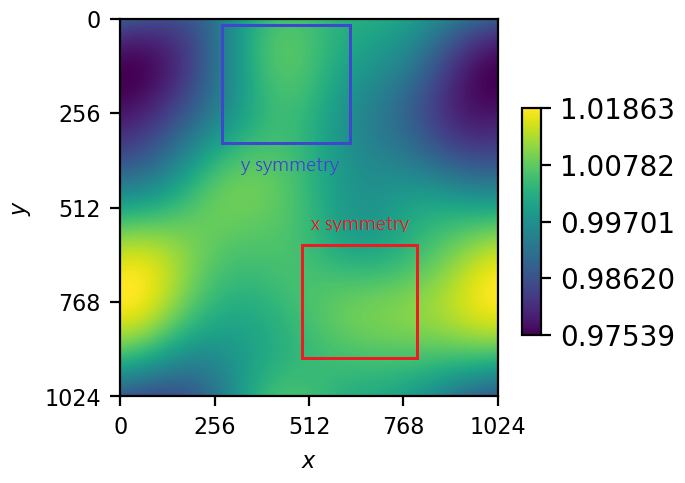
\includegraphics[width=13cm]{x_symmetry_and_y_symmetry_text.png} %[]可選參數,控制圖片大小
%圖片說明
\caption{Regions Might Possess $x$ or $y$ Symmetry}
\end{figure}

\begin{figure}[htbp] %htbp 代表图片插入位置的设置
\centering %圖片置中
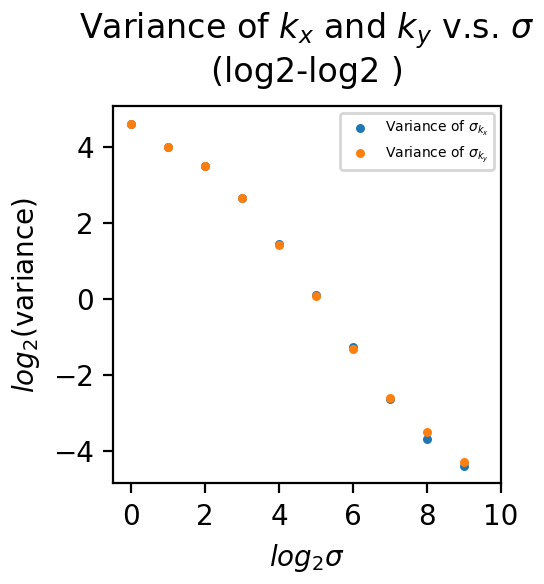
\includegraphics[width=10cm]{log2-log2_variance_v.s._sigma.png} %[]可選參數,控制圖片大小
%圖片說明
\caption{log2-log2 variance v.s. $\sigma$}
\end{figure}



\end{large}
\end{document}
